\chapter{The Basics}
\section{Graphs and subgraphs}

In this chapter, we will introduce to the reader some basic definitions and notation in graph theory, which will be used throughout this thesis. We will follow \citeauthor{diestel00}'s book \textit{Graph Theory} for these standard definitions and notation.

Now, let us start with the definition of a graph. Informally, a \textit{graph} is a set of vertices and edges, where the edges connect some of the vertices in the set. The letter $u$ and $v$ are the most commonly used notation for vertices, and $e$ is also commonly used to denote an edge of a graph, where in this case the two vertices connected by the edge $e$ is unspecified. We say a vertex $v$ is incident to an edge $e$ if $e$ is an edge at $v$. We also denote the edge $e$ by $uv$ if the vertices $u$ and $v$ are both incident to $e$. In this case $u$ and $v$ are called the {\it {ends}} of the edge $e$. We now give a more precise definition of a graph. A {\it{graph}} is an ordered pair $G = (V(G), E(G))$, where $V(G)$ and $E(G)$ denote the sets of  vertices and edges of the graph $G$ respectively. We say a graph is a \emph{simple graph} if it does not contain a loop between a pair of vertices. The following are two examples of graphs. In the first case (Fig. \ref{graph} (a)), the graph is connected (contains only one component), while in the second case (Fig. \ref{graph} (b)), the graph is disconnected. A formal definition of a connected graph will be given in the next section. 
\begin{figure}
  \centering
     % \vspace{-10pt}
    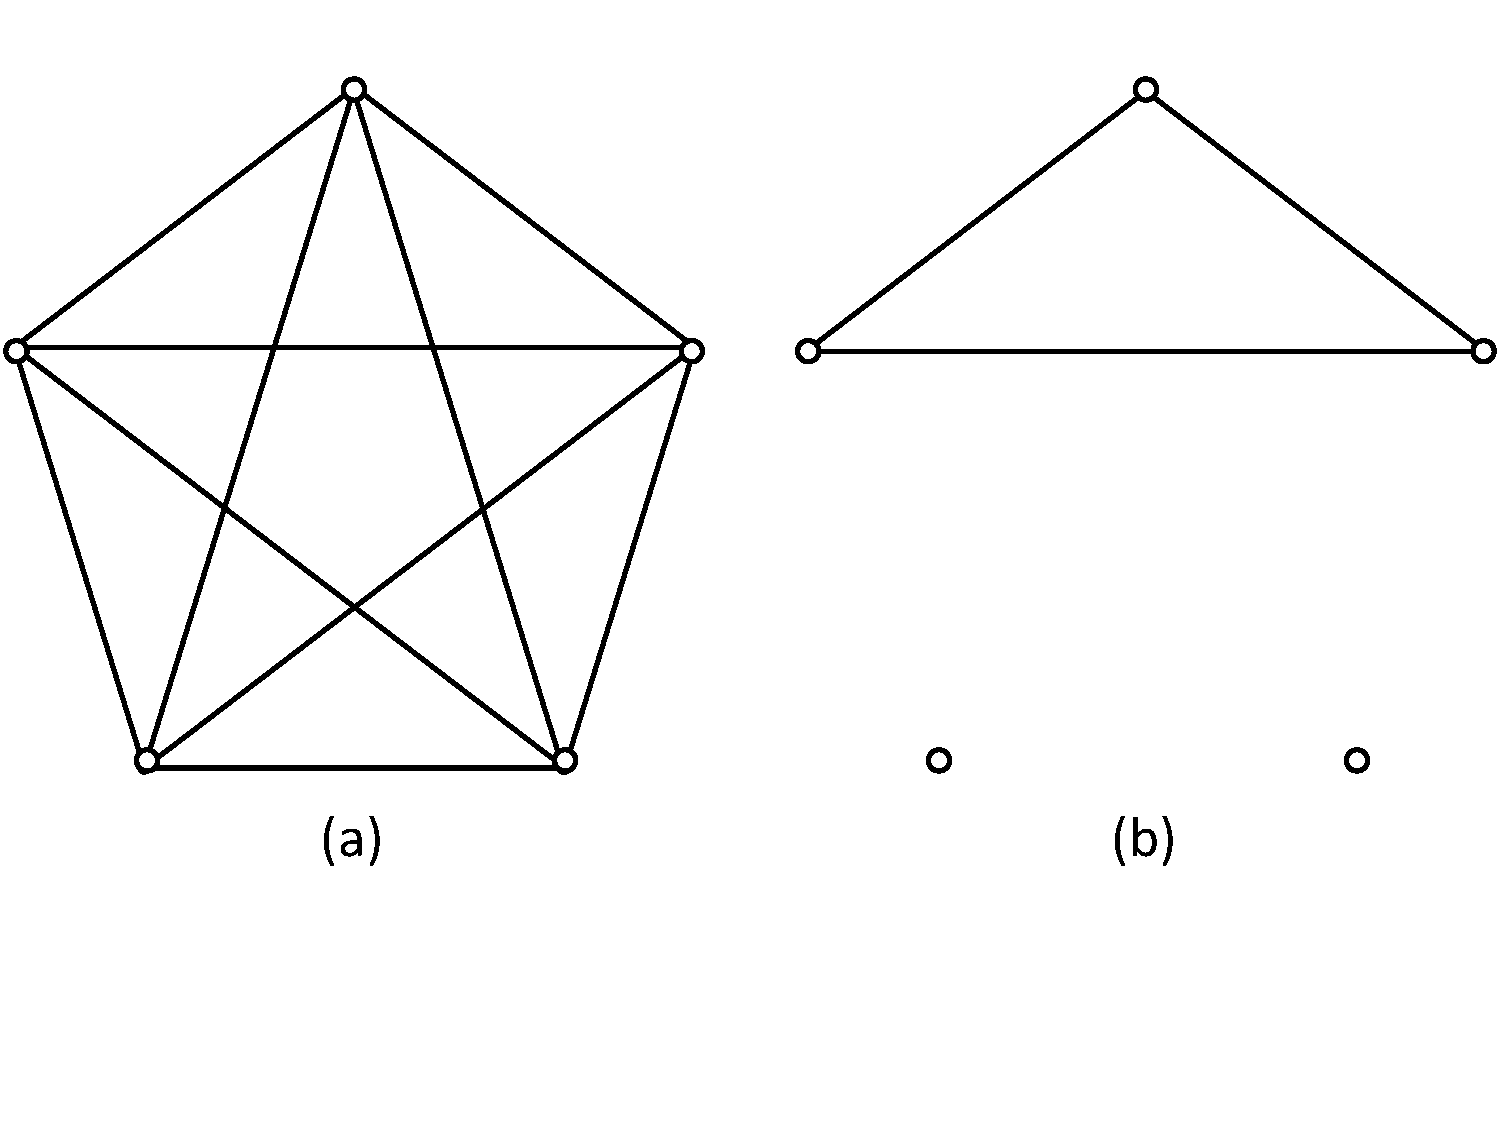
\includegraphics[scale=0.35]{../figures/fig2-1.pdf}
        \vspace{-30pt}
  \caption{Example of graphs}
  \label{graph}
\end{figure}

Since $V(G)$ and $E(G)$ denote the sets of vertices and edges of the graph $G$, there must be subsets of $V(G)$ and $E(G)$. This brings in the following definition. A graph $G' = (V'(G), E'(G))$ is a {\it{subgraph}} of a graph $G = (V(G), E(G))$ if $V'(G) \subseteq V(G)$ and $E'(G) \subseteq E(G)$ are subsets. We use $G' \subseteq G$ to denote $G'$ is a subgraph of $G$. Sometimes we also say that the graph $G$ contains $G'$ as a subgraph.  For the two graphs below (Fig \ref{graph}), clearly (b) is a subgraph of (a). 

The {\it{degree}} of a vertex $v$ in a graph $G$ is the number of vertices adjacent to $v$. It is denoted by $d_G(v)$ or $d(v)$.\footnote{This notation, as well as others, are widely used throughout this thesis. For convenience, we drop the index $G$ if $G$ is clearly understood.}  Equivalently, it can be defined as the number of edges incident to $v$. In Fig \ref{graph} (b), the bottom left vertex has degree $0$. The top  vertex has degree $2$. Sometime we use $\Delta(G)$ (or just $\Delta$) to denote the maximum degree of a graph $G$. Precisely, $\Delta(G) := \max_{u \in V(G)} d(u)$. 


%%%%%%%%%%%%%%%%%%%%%%%%
\section{Paths, cycles and trees}
Intuitively, a path is a finite series of edges between a pair of vertices. To make it more formal, we define a {\it {path}} $P = (V, E)$ as a subgraph of a simple graph $G$, where the set $V = \{x_0, x_1, \dots, x_n\}$ and the set $E = \{x_0x_1, x_1x_2, \dots, x_{n-1}x_n\}$. The {\it{length}} of $P$ is said to be the number of edges in $P$. A path $P$ of length $n$ is normally denoted by $P^n$. Notice that for vertices $x_0$ and $x_n$ of a graph, there could be more than one path between them. Hence we use $P = x_0x_1\dots x_{n-1}x_n$ referring to the particular path that we are interested in. We call a path $P$ from $x_0$ to $x_n$ that has the least length the {\it{shortest path}} between $x_0$ and $x_n$. Though the length of such a path is the least among all other paths from $x_0$ to $x_n$, the shortest path between $x_0$ and $x_n$ is not unique in some graphs. We use the length of the shortest path between two vertices $x_0$ and $x_n$ to define the {\it{distance}} between $x_0$ and $x_n$ in a graph $G$, denoted by $dis_G(x_0,x_n)$ or $dis(x_0,x_n)$ or $d(x_0,x_n)$. On the other hand, the \textit{diameter} of a graph $G$, denoted by $diam(G)$ is the length of the longest path in $G$. 

We call a path with the two ends are identical a \textit{cycle}, denoted by $C = x_0x_1\dots x_nx_0$. In other words, a cycle is a closed path. The \emph{length} of a cycle is defined to be the number of vertices or edges in it. A cycle $C$ of length $n$ is said to be an {\it{$n$-cycle}} and denoted by $C^n$.

Let us use the following example to make the above definitions clear. 

\begin{example}
Let $G$ be a graph as shown in Fig. \ref{path and cycle}. Then $P = x_0x_1x_2x_3x_4$ is a path of length $4$ in $G$, and $C =  x_0x_1x_2x_3x_4x_0$ is a cycle of length $5$ in $G$. Also, the distance between $u_0$ and $u_4$ in $G$ is $1$, as there is a shortest path $u_0u_1$ of length $1$ in $G$. 

\begin{figure}
  \centering
      \vspace{-10pt}
    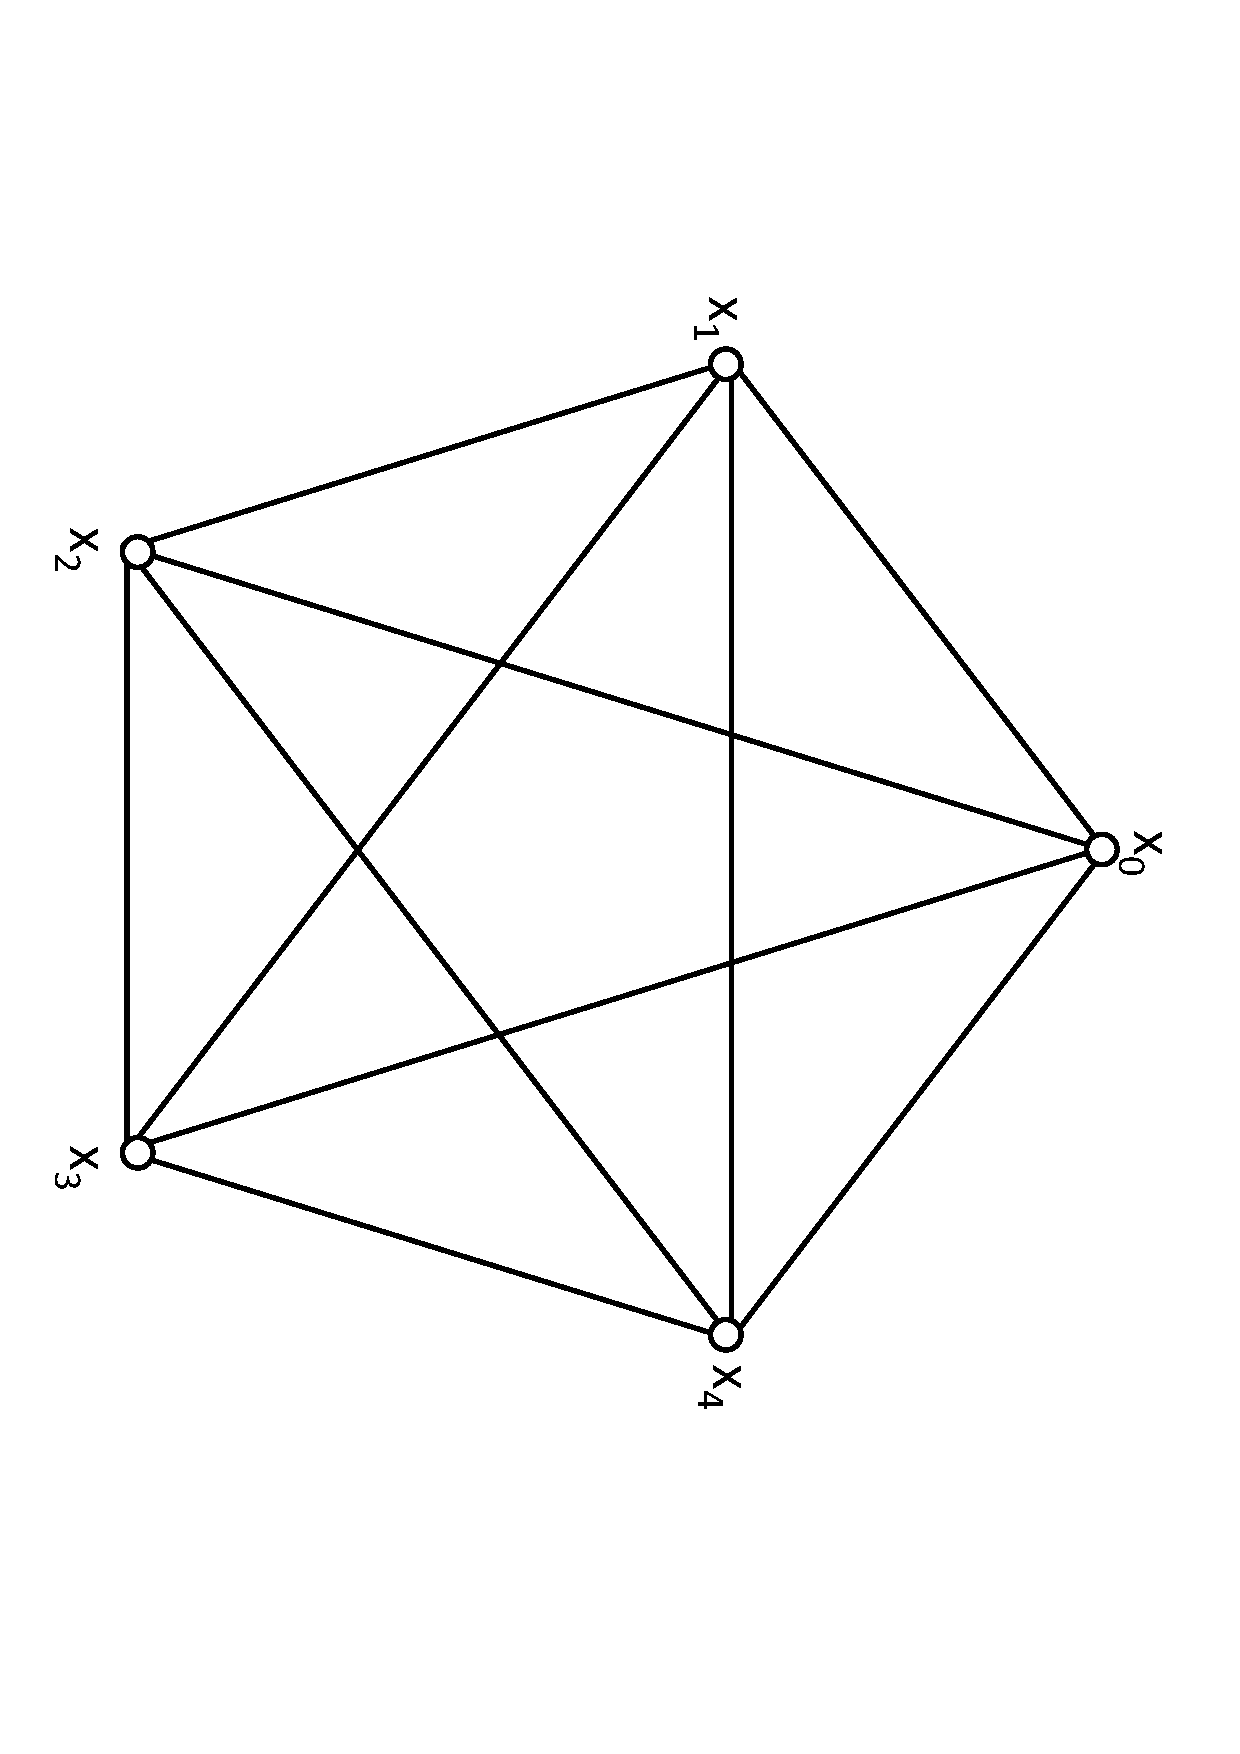
\includegraphics[scale=0.25, angle=90]{../figures/fig2-2.pdf}
        \vspace{5pt}
  \caption{Example of a path and a cycle}
  \label{path and cycle}
\end{figure}

\end{example}

Any graph $G$ may or may not contain a cycle as a subgraph. We say a graph is {\it{acyclic}} if it does not contain a cycle. 

A \emph{component} of a graph is an isolated block that is not connected to any other vertices or edges of the graph. A graph is {\it{connected}} if it has only one component. On the other hand, if a graph contains more than one component, then we say such a graph is not connected or {\it{disconnected}}. We have seen examples of connected and disconnected graphs previously (Fig \ref{graph}). 

Using the above definitions, we can give a formal definition of trees. A {\it{tree}} is defined as a connected acyclic graph. Normally, we use $T$ to denote a tree. For instance, a path is a tree. If a graph is acyclic but not connected, then it contains more than one tree. Such a graph is said to be a {\it{forest}}. When dealing problems with a tree, it is convenient to have a special vertex. Such a vertex is called the \emph{root} of this tree. A tree with a fixed root is called a {\it{rooted tree}}. Notice that we can only make one special vertex in each tree. In other words, there is only one root in each rooted tree. All trees that are dealt with in this thesis are rooted trees, so in future we will only say a tree $T$ instead of a rooted tree $T$ just for convenience. A {\it{leaf}} of a tree is a non-rooted vertex such that the degree of the vertex is exactly one. We say vertices of a tree $T$ are \textit{internal vertices} if they are not leaves of $T$. The root of $T$ is also an internal vertex of $T$. The {\it{parent}} of a vertex $v$ in a tree $T$ is a vertex that is connected to $v$ on the path from $v$ to the root of $T$, denoted by $P(v)$. The parent $P(v)$ in a tree $T$ is unique, since there is a unique path between any two vertices of $T$ and the parent of $v$ is on this unique path. We will prove this in the following proposition. The {\it{child}} of a vertex $v$ in $T$ is defined as a vertex that is adjacent to $v$ on the path from $v$ to a leaf of $T$, denoted by $C(v)$. Unlike the parent, a vertex $v$ can have more than one child if there is more than one leaf in $T$. 

Here, we introduce another concept, the \emph{neighbours} of a vertex $u \in V(G)$, which is the set of vertices adjacent to $u$. Precisely, we have the following definition. 

\begin{definition}
\label{neighbour}
Let $u \in V(G)$ be a vertex of a graph $G$. We define the set of neighbours of $u$ to be  
\[
N(u) := \{v \in V(G) \mid d(u,v) = 1\}.
\]
\end{definition}

Intuitively, if we have a tree, we can ask the height of such a tree. The length of the longest path from the root of $T$ to leaves of $T$ is defined to be the {\it{height}} of a tree $T$ and denote it by $hei(T)$. For any vertex $u$ in a tree $T$, we can also talk about its {\it{depth}}. It is defined as the length of the path from the root of $T$ to any vertex $u$ of $T$, denoted by $dep_T(u)$. This is well-defined because there is a unique path from the root to any vertex of $T$. Precisely, we have the following proposition. 

\begin{proposition}
\label{prop:unique path}
Let $T$ be a tree. There is a unique path between any two vertices $u, v \in V(T)$. 
\end{proposition}

\begin{proof}
The proof of this proposition is straightforward. Let $P$ be a path in the tree $T$ from $u$ to $v$. Suppose there is another path $P'$ in $T$ from $u$ to $v$ such that $P \neq P'$. Since both paths have end points $u$ and $v$, there eixsts a cycle in $T$ passes through $u$ and $v$. But $T$ is acyclic by the definition of a tree, so we must have $P=P'$.
\end{proof}
\qed

If we let $u$ to be the root of $T$, then the proposition claims there is a unique path between the root of $T$ and any other vertex in $T$. Due to the uniqueness of a path in trees, we can use $P_{uv}$ to denote the unique path from vertex $u$ to $v$ in a tree $T$ for convenience. 

\begin{example}
In Fig. \ref{height and depth}, the tree $T$ has height $4$, as $P_{uw}$ is the longest path from the root of $T$ to its leaves, and it has length $4$. Also, $dep(v) = 3$ as the length of the path $P_{uv}$ is $3$. 

\begin{figure}
  \centering
      \vspace{-10pt}
    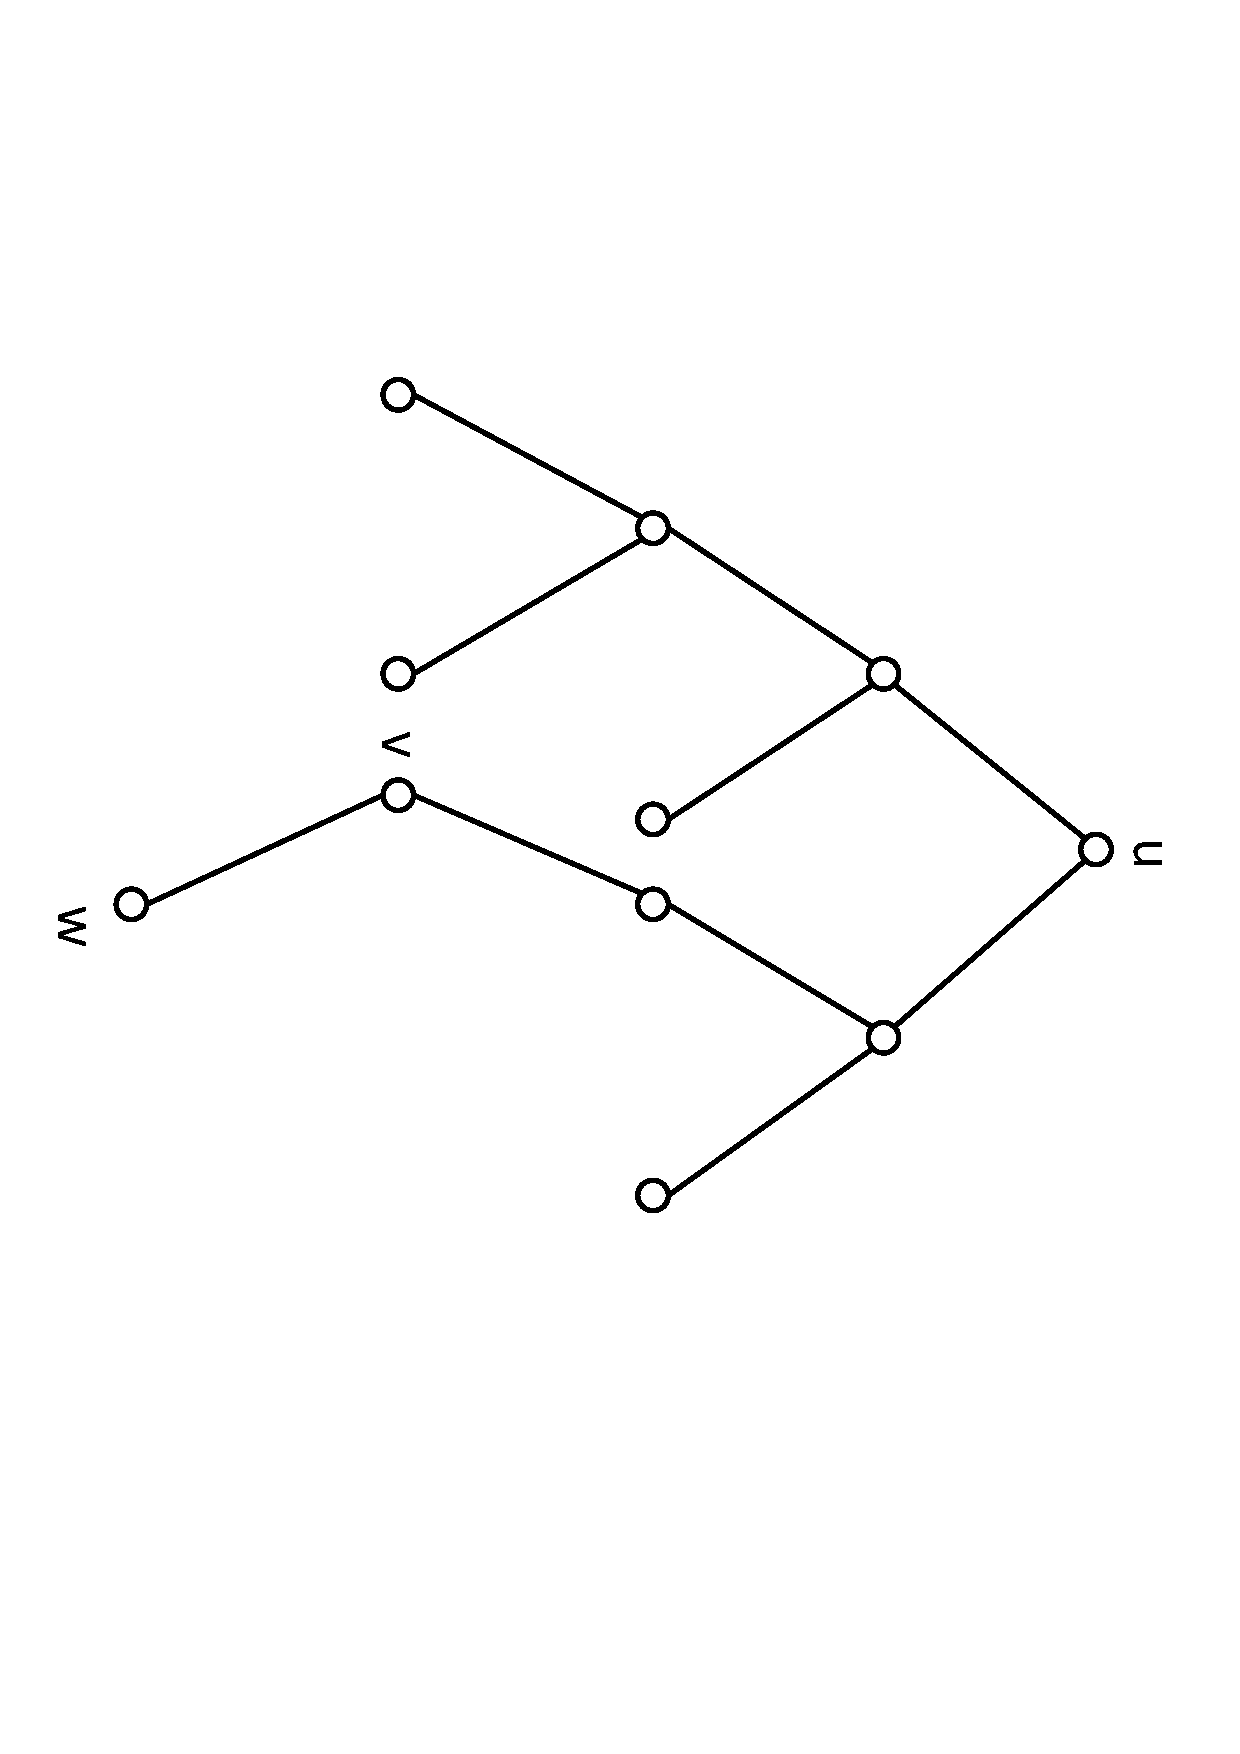
\includegraphics[scale=0.3, angle=90]{../figures/fig2-3.pdf}
        \vspace{-0pt}
  \caption{Tree height and vertex depth}
  \label{height and depth}
\end{figure}
\end{example}

%%%%%%%%%%%%%%%%%%%%%%%%%%%%%%%%%%%%%

\section{Complete $m$-ary trees}
Our research begins with labelling the set of complete $m$-ary trees. We now give the formal definition of a complete $m$-ary tree. 
\begin{definition}
\label{m-ary tree}
A tree $T$ is said to be an $m$-ary tree if every internal vertex  of $T$ has exactly $m$ children, for $m \in \mathbb{N}$.\footnote{In this thesis, we define $\mathbb{N}:=\{0, 1, \dots\}$ non-negative integers}Moreover, if all leaves in an $m$-ary tree $T$ have the same depth then we say $T$ is a complete $m$-ary tree. 
\end{definition}

The height of a complete $m$-ary tree is also the depth of any leaf of it.  Throughout this thesis, we will denote a complete $m$-ary tree with height $k$ by $\tmk$, for $m, k$ are non-negative integers. 

A trivial example of a complete $m$-ary tree is a single vertex. It is a complete $0$-ary tree. Here is another example. 
\begin{example}
In Fig. \ref{example of m-ary tree}, both (a) and (b) are $2$-ary trees with height $k = 2$. The $2$-ary tree in (a) is not complete, while the one in (b) is a complete $2$-ary tree. 

\begin{figure}
\centering
      \vspace{-15pt}
    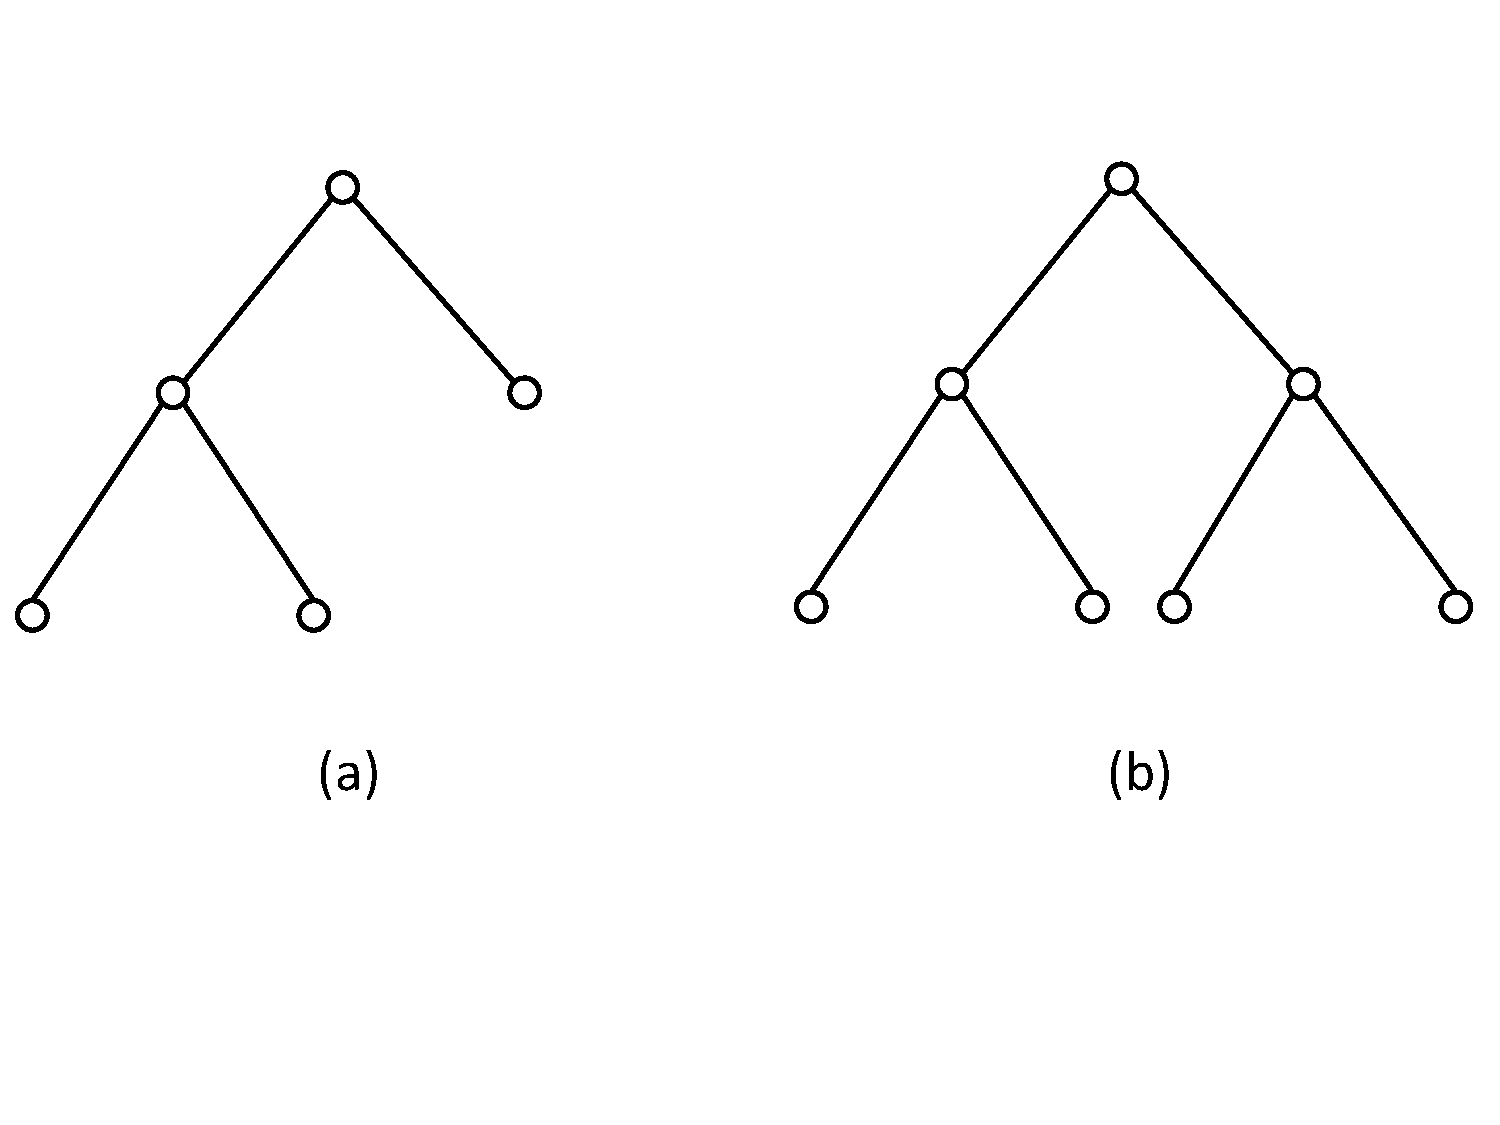
\includegraphics[scale=0.4]{../figures/fig2-4.pdf}
        \vspace{-50pt}
\caption{Example of $m$-ary trees}
\label{example of m-ary tree}
\end{figure}

\end{example}

As we mentioned in Chapter 1, this thesis will only deal with graph labelling problems with distance three constraint. For a complete $m$-ary tree $\tmk$ to be eligible for distance three labelling, we require the diameter of $\tmk$ to be no less than $3$. Thus, the height $k$ of $\tmk$ needs to be at least $2$, and the number of children $m$ of each vertex needs also to be at least $2$. In other words, all the complete $m$-ary trees $\tmk$ in this these have $k \ge 2$ and $m \ge 2$. Throughout the thesis we will now assume that these conditions are satisfied. 

The next remark shows how to construct a complete tree with height $k+1$ from complete $m$-ary tree with height $k$. 
 
\begin{remark}
\label{construct}
Take $m$ copies of a complete $m$-ary tree $\tmk$ and name the root of each single copy $u_0^i$, where $i \in [1,m]$. Connect each $u_0^i$ by an extra edge to the new vertex $u_0^0$. (Fig. \ref{example of construct}) The resulted graph is a complete $m$-ary tree with height $k+1$. The root of this larger complete $m$-ary tree $T_{m,k+1}$ is $u_0^0$. 

\begin{figure}
\centering
      \vspace{-0pt}
    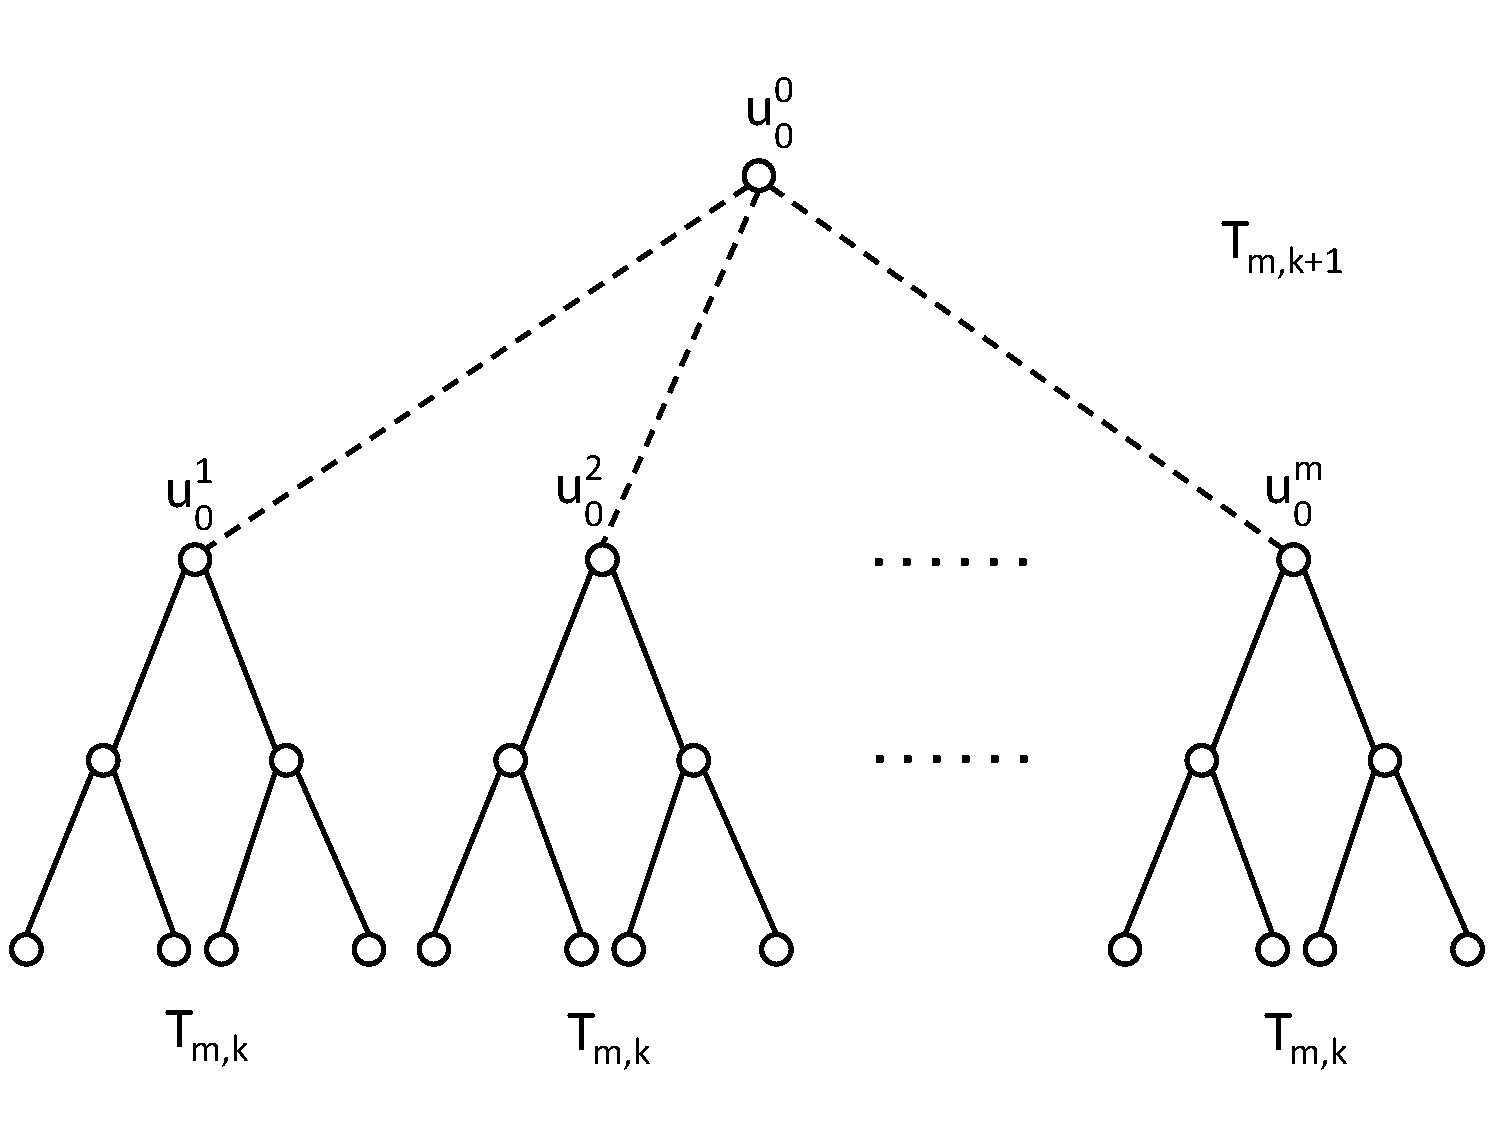
\includegraphics[scale=0.4]{../figures/fig2-5.pdf}
        \vspace{-0pt}
\caption{Construct $T_{m,k+1}$ from $\tmk$}
\label{example of construct}
\end{figure}
\end{remark}

Now, we have finished introducing most of the definitions that will be used throughout this thesis. It is time to start presenting our results.







